%!TEX root = ../main.tex

%
%

\chapter{Math fundamentals}
\label{chapter:math_fundamentals}

In this chapter we'll review the fundamental ideas of mathematics, including numbers, equations, and functions.  
To understand college-level textbooks, you need to be comfortable with mathematical calculations.
Many people have trouble with math, however. 
Some people say they \emph{hate} math, or could never learn it. 
It's not uncommon for children who score poorly on their school math exams to develop math complexes in their grown lives.
If you are carrying any such emotional baggage, you can drop it right here and right now.

Do NOT worry about math! 
You are an adult, and you can learn math much more easily than when you were a kid.
We'll review \emph{everything} you need to know about high school math, and by the end of this chapter, 
you'll see that math is nothing to worry about.

\smallskip

\begin{figure}[H]
\centering
\! 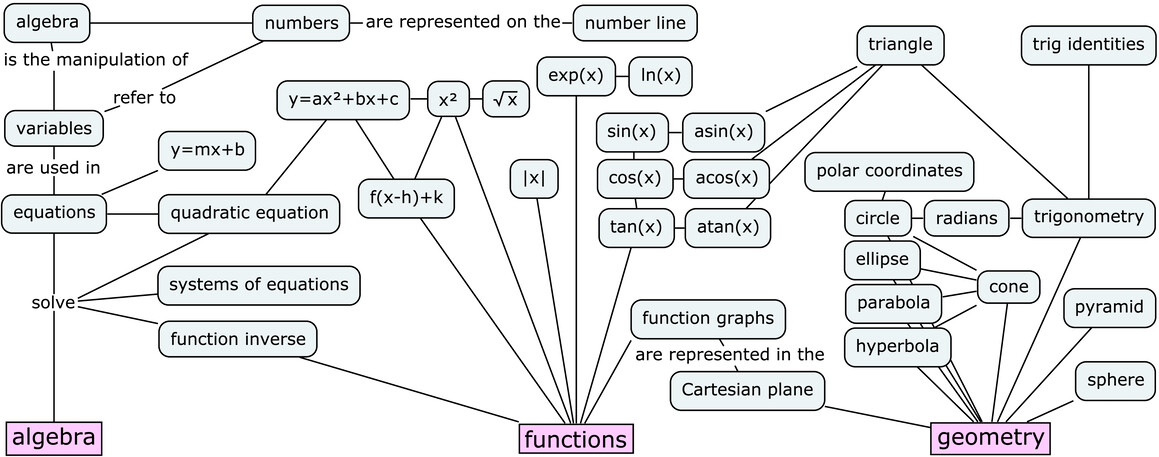
\includegraphics[width=1.01\textwidth]{images/figures/concept_maps/precalculus.jpg}
	\caption{A concept map showing the mathematical topics that we will cover in this chapter.
			We'll learn how to solve equations using algebra, 
			how to model the world using functions,
			and how to think geometrically.
			The material in this chapter is required for your understanding of the more advanced topics in this book.\label{fig:precalculus_concept_map}}

\end{figure}

\section{Solving equations}
\label{sec:solving_equations}
	
	Most math skills boil down to being able to manipulate and solve equations.
	Solving an equation means finding the value of the unknown in the equation.  

	Check this \pgt{}{shit} out:
	\[
	 x^2-4=45.
	\]
	To solve the above equation is to answer
	the question ``What is $x$?''
	More precisely, we want to find the number that can take the 
	place of $x$ in the equation so that the equality holds.
	In other words, we're asking,
	\[
	  \text{``Which number times itself minus four gives 45?''}
	\]
	That is quite a mouthful, don't you think? 
	To remedy this verbosity, mathematicians often use specialized symbols to describe math operations.
	The problem is that these specialized symbols can be very confusing. 
	Sometimes even the simplest math concepts are inaccessible if you don't know what the symbols mean. 

	What are your feelings about math, dear reader? Are you afraid of it? 
	Do you have anxiety attacks because you think it will be too difficult for you?
	Chill! Relax, my brothers and sisters. There's nothing to it.
	Nobody can magically guess the solution to an equation immediately.
	To find the solution, you must break the problem into simpler steps.
	Let's walk through this one together.

	To find $x$, we can manipulate the original equation, 
	transforming it into a different equation (as true as the first) that looks like this:
	\[
	  x \; = \textrm{ only numbers.}
	\]

	\noindent
	That's what it means to \emph{solve} an equation:
	the equation is solved because the unknown is isolated on one side,
	while the constants are grouped on the other side.
	You can type the numbers on the right-hand side into a calculator and obtain the numerical value of $x$.

	By the way, before we continue our discussion,
	let it be noted: the equality symbol ($=$) means that all that is to the left of $=$ 
	is equal to 
	all that is to the right of $=$. 
	To keep this equality statement true,  
	\textbf{for every change you apply to the left side of the equation, 
	you must apply the same change to the right side of the equation}.

		To find $x$,
	we need to manipulate the original equation into its final form,
	simplifying it step by step until it can't be simplified any further.
	The only requirement is that the manipulations we make transform one true equation into another true equation.
	In this example,
	the first simplifying step is to add the number four to both sides of the equation:
	\[
	 	x^2-4  \; + 4  	=	45    \; + 4, 	    \\
	\]
	which simplifies to
	\[
		x^2 	 		=	49.
	\]
	Now the expression looks simpler, yes?
	How did I know to perform this operation? 
	I wanted to ``undo'' the effects of the operation $-4$.
	We undo an operation by applying its \emph{inverse}.
	In the case where the operation is the subtraction of some amount,
	the inverse operation is the addition of the same amount.

	We're getting closer to our goal of \emph{isolating} $x$ on one side of the equation,							
	leaving only numbers on the other side.
	The next step is to undo the square $x^2$ operation.
	The inverse operation of squaring a number $x^2$ is to take its square root $\sqrt{\phantom{a}\; }$,
	so that's what we'll do next. We obtain
	\[ 
	   \sqrt{x^2} 		= 	\sqrt{49}.
	\]
	Notice how we applied the square root  to both sides of the equation? 
	If we don't apply the same operation to both sides, we'll break the equality!

	The equation $\sqrt{x^2}= \sqrt{49}$ simplifies to 
	\[
	 	|x|	= 	7.
	 \]
	What's up with the vertical bars around $x$?
	The notation $|x|$ stands for the \emph{absolute value} of $x$,											
	which is the same as $x$ except we ignore the sign that indicates whether $x$ is positive or negative. 
	For example $|5|=5$ and $|-5|=5$, too.
	The equation $|x|=7$ indicates that both $x=7$ and $x=-7$ satisfy the equation $x^2 = 49$.
	Seven squared is 49, $7^2=49$, and negative seven squared is also 49, $(-7)^2 = 49$,
	because the two negative signs cancel each other out.

	The final solutions to the equation $x^2-4=45$ are													
	\[
	 x  = 7 \qquad \textrm{and} \qquad   x=  - 7.
	\]
	Yes, there are \emph{two} possible answers. 
	You can check that both of the above values of $x$ satisfy the initial equation $x^2-4=45$.

	\bigskip

	If you are comfortable with all the notions of high school math
	and you feel you could have solved the equation $x^2-4=45$ on your own,			then you can skim through this chapter quickly.
	If on the other hand you are wondering how the squiggle killed the power two,
	then this chapter is for you!
	In the following sections we will review all the essential concepts from
	high school math that you will need to power through the rest of this book.
	First, let me tell you about the different kinds of numbers.


\section{Numbers}
\label{sec:numbers}

	In the beginning, we must define the main players in the world of math: numbers.

	\subsection{Definitions}
	\label{numbers:definitions}
		
		Numbers are the basic objects we use to count, measure, quantify, and calculate things.
		Mathematicians like to classify the different kinds of number-like objects into categories called \emph{sets}:					
		\begin{itemize}
			\item  The natural numbers: $\mathbb{N} = \{0,1,2,3,4,5,6,7, \ldots \, \}$
			\item  The integers: $\mathbb{Z} = \{\ldots, -3,-2,-1,0,1,2,3 , \ldots  \, \}$
			\item  The rational numbers: $\mathbb{Q} = \{\frac{5}{3}, \frac{22}{7}, 1.5, 0.125,  -7, \, \ldots \, \}$
			\item  The real numbers: $\mathbb{R} = \{-1,0,1, \sqrt{2}, e,\pi, \;  4.94\ldots, \; \ldots \, \}$
			\item  The complex numbers: $\mathbb{C} = \{ -1, 0, 1, i,  1+i, 2+3i,  \ldots \, \}$
		\end{itemize}
				These categories of numbers should be somewhat familiar to you.
		Think of them as neat classification labels for everything that you would normally call a number. 
	 	Each group in the above list is a \emph{set}.
		A set is a collection of items of the same kind. 
		Each collection has a name and a precise definition for which items belong in that collection.
		Note also that each of the sets in the list contains all the sets above it,												
		as illustrated in Figure~\ref{fig:nested_sets}.
		For now, we don't need to go into the details of sets and set notation,
		but we do need to be aware of the different sets of numbers.

		\begin{figure}[H]
			\centering
			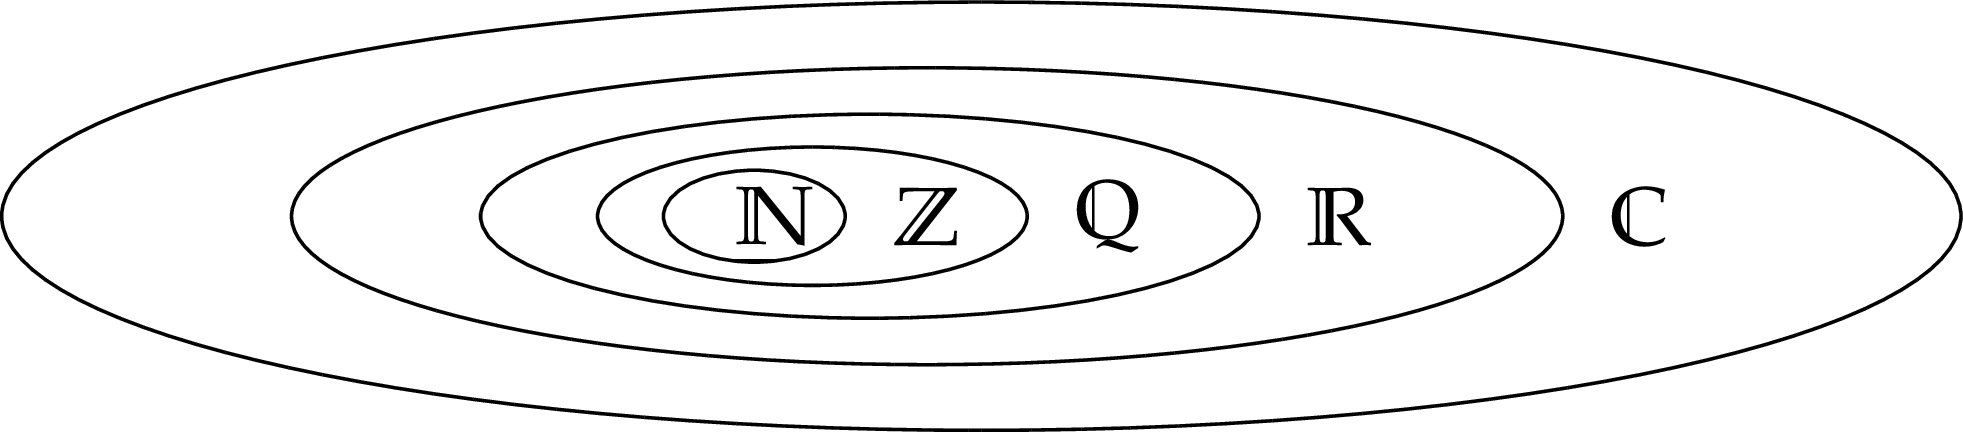
\includegraphics[width=0.87\textwidth]{images/figures/math/nested_sets.png}
			\caption{	An illustration of the nested containment structure of the different number sets.
					The set of natural numbers is contained in the set of integers,
					which in turn is contained in the set of rational numbers.
					The set of rational numbers is contained in the set of real numbers,
					which is contained in the set of complex numbers.\label{fig:nested_sets}}
			
		\end{figure}

		\noindent
		Why do we need so many different sets of numbers?
		Each set of numbers is associated with more and more advanced mathematical problems.

		The simplest numbers are the natural numbers $\mathbb{N}$,
		which are sufficient for all your math needs if all you're going to do is \emph{count} things.
		How many goats? Five goats here and six goats there so the total is 11 goats. 
		The sum of any two natural numbers is also a natural number.

		As soon as you start using \emph{subtraction} (the inverse operation of addition),
		you start running into negative numbers,
		which are numbers outside the set of natural numbers.
		If the only mathematical operations you will ever use are \emph{addition} and \emph{subtraction},
		then the set of integers $\mathbb{Z} = \{ \ldots, -2, -1, 0, 1, 2, \ldots \}$ will be sufficient.
		Think about it.
		Any integer plus or minus any other integer is still an integer.

		You can do a lot of interesting math with integers.
		There is an entire field in math called \emph{number theory} that deals with integers.
		However, to restrict yourself solely to integers is somewhat limiting---a rotisserie
		menu that offers $\frac{1}{2}$ of a chicken would be totally confusing.

		If you want to use division in your mathematical calculations,														
		you'll need the rationals~$\mathbb{Q}$.
		The set of rational numbers corresponds to all numbers that can be expressed as \emph{fractions} of the form $\frac{m}{n}$		
		where $m$ and $n$ are integers, and $n \neq 0$.
		You can add, subtract, multiply, and divide rational numbers, and the result will always be a rational number.
		However, even the rationals are not enough for all of math!

		In geometry, we can obtain \emph{irrational} quantities like $\sqrt{2}$ (the diagonal of a square with side 1)
		and $\pi$ (the ratio between a circle's circumference and its diameter).
		There are no integers $x$ and $y$ such that $\sqrt{2}=\frac{x}{y}$,
		therefore we say that $\sqrt{2}$ is \emph{irrational} (not in the set $\mathbb{Q}$).
		An irrational number has an infinitely long decimal expansion that doesn't repeat.
		For example, $\pi = 3.141592653589793\ldots$ where the dots indicate
		that the decimal expansion of $\pi$ continues all the way to infinity.

		Combining the irrational numbers with the rationals gives us all the useful numbers,
		which we call the set of real numbers $\mathbb{R}$.
		The set $\mathbb{R}$ contains the integers,
		the rational numbers $\mathbb{Q}$,
		as well as irrational numbers like $\sqrt{2}=1.4142135\ldots$.
		By using the reals you can compute pretty much anything you want.
		From here on in the text, when I say \emph{number},
		I mean an element of the set of real numbers $\mathbb{R}$.

		The only thing you can't do with the reals is to take the square root of a negative number---you 							
		need the complex numbers $\mathbb{C}$ for that.
		We defer the discussion on $\mathbb{C}$ until the end of Chapter~\ref{chapter:vectors}.


	\subsection{Exercises}
	\label{numbers:exercises}
	
		%!TEX root = ../main.tex

\begin{exercises}{ch1}	


	\begin{exercise}
		Solve for the unknown $x$ in the following equations:

		\twocol
		\textbf{a)}~$3x+2-5=4+2$

		\textbf{b)}~$\frac{1}{2}x-3=\sqrt{3}+12-\sqrt{3}$
		\endtwocol

		\twocol
		\textbf{c)}~$\frac{7x-4}{2} +1 = 8-2$
		
		\textbf{d)}~$5x-2+3=3x-5$
		\endtwocol
				
		\begin{eanswer}\textbf{a)}~$x=3$; \textbf{b)}~$x=30$; \textbf{c)}~$x=2$; \textbf{d)}~$x=-3$.\end{eanswer}
					\end{exercise}


	\begin{exercise}
		Indicate all the number sets the following numbers belong to.
				
		\fivecol
		\textbf{a)}~$-2$ 

		\textbf{b)}~$\sqrt{-3}$
		
		\textbf{c)}~$8 \div 4$
		
		\textbf{d)}~$\frac{5}{3}$
		
		\textbf{e)}~$\frac{\pi}{2}$
		
		\endfivecol
		
		\begin{eanswer}\textbf{a)}~$\mathbb{Z}, \mathbb{Q}, \mathbb{R},\mathbb{C}$;
					\textbf{b)}~$\mathbb{C}$;
					\textbf{c)}~$\mathbb{N},\mathbb{Z}, \mathbb{Q}, \mathbb{R},\mathbb{C}$;
					\textbf{d)}~$\mathbb{Q}, \mathbb{R},\mathbb{C}$;
					\textbf{e)}~$\mathbb{R},\mathbb{C}$.\end{eanswer}
					\end{exercise}

	

	\begin{exercise}
		Calculate the values of the following expressions:
		
		\threecol
		\textbf{a)}~$2^33-3$ 

		\textbf{b)}~$2^3(3-3)$
		
		\textbf{c)}~$\frac{4-2}{3^3}(6\cdot 7- 41)$
		\endthreecol
		
		\begin{eanswer}\textbf{a)}~$21$; \textbf{b)}~$0$; \textbf{c)}~$\frac{2}{27}$.\end{eanswer}
					\end{exercise}	



\end{exercises}

	


\section{Hyperbola}
\label{sec:hyperbola}

	The \emph{hyperbola} is another fundamental shape of nature.
	

	\subsection{The conic sections}

		There is a deep connection between the geometric shapes of the circle,
		the ellipse, the parabola, and the hyperbola.
		These seemingly different shapes can be obtained, geometrically speaking,
		from a single object: the cone.															
		We can obtain the four curves by slicing the cone at different angles,
		as illustrated in Figure~\ref{fig:conic_sections_four-shapes}.

		\begin{figure}[htb]
			\centering
			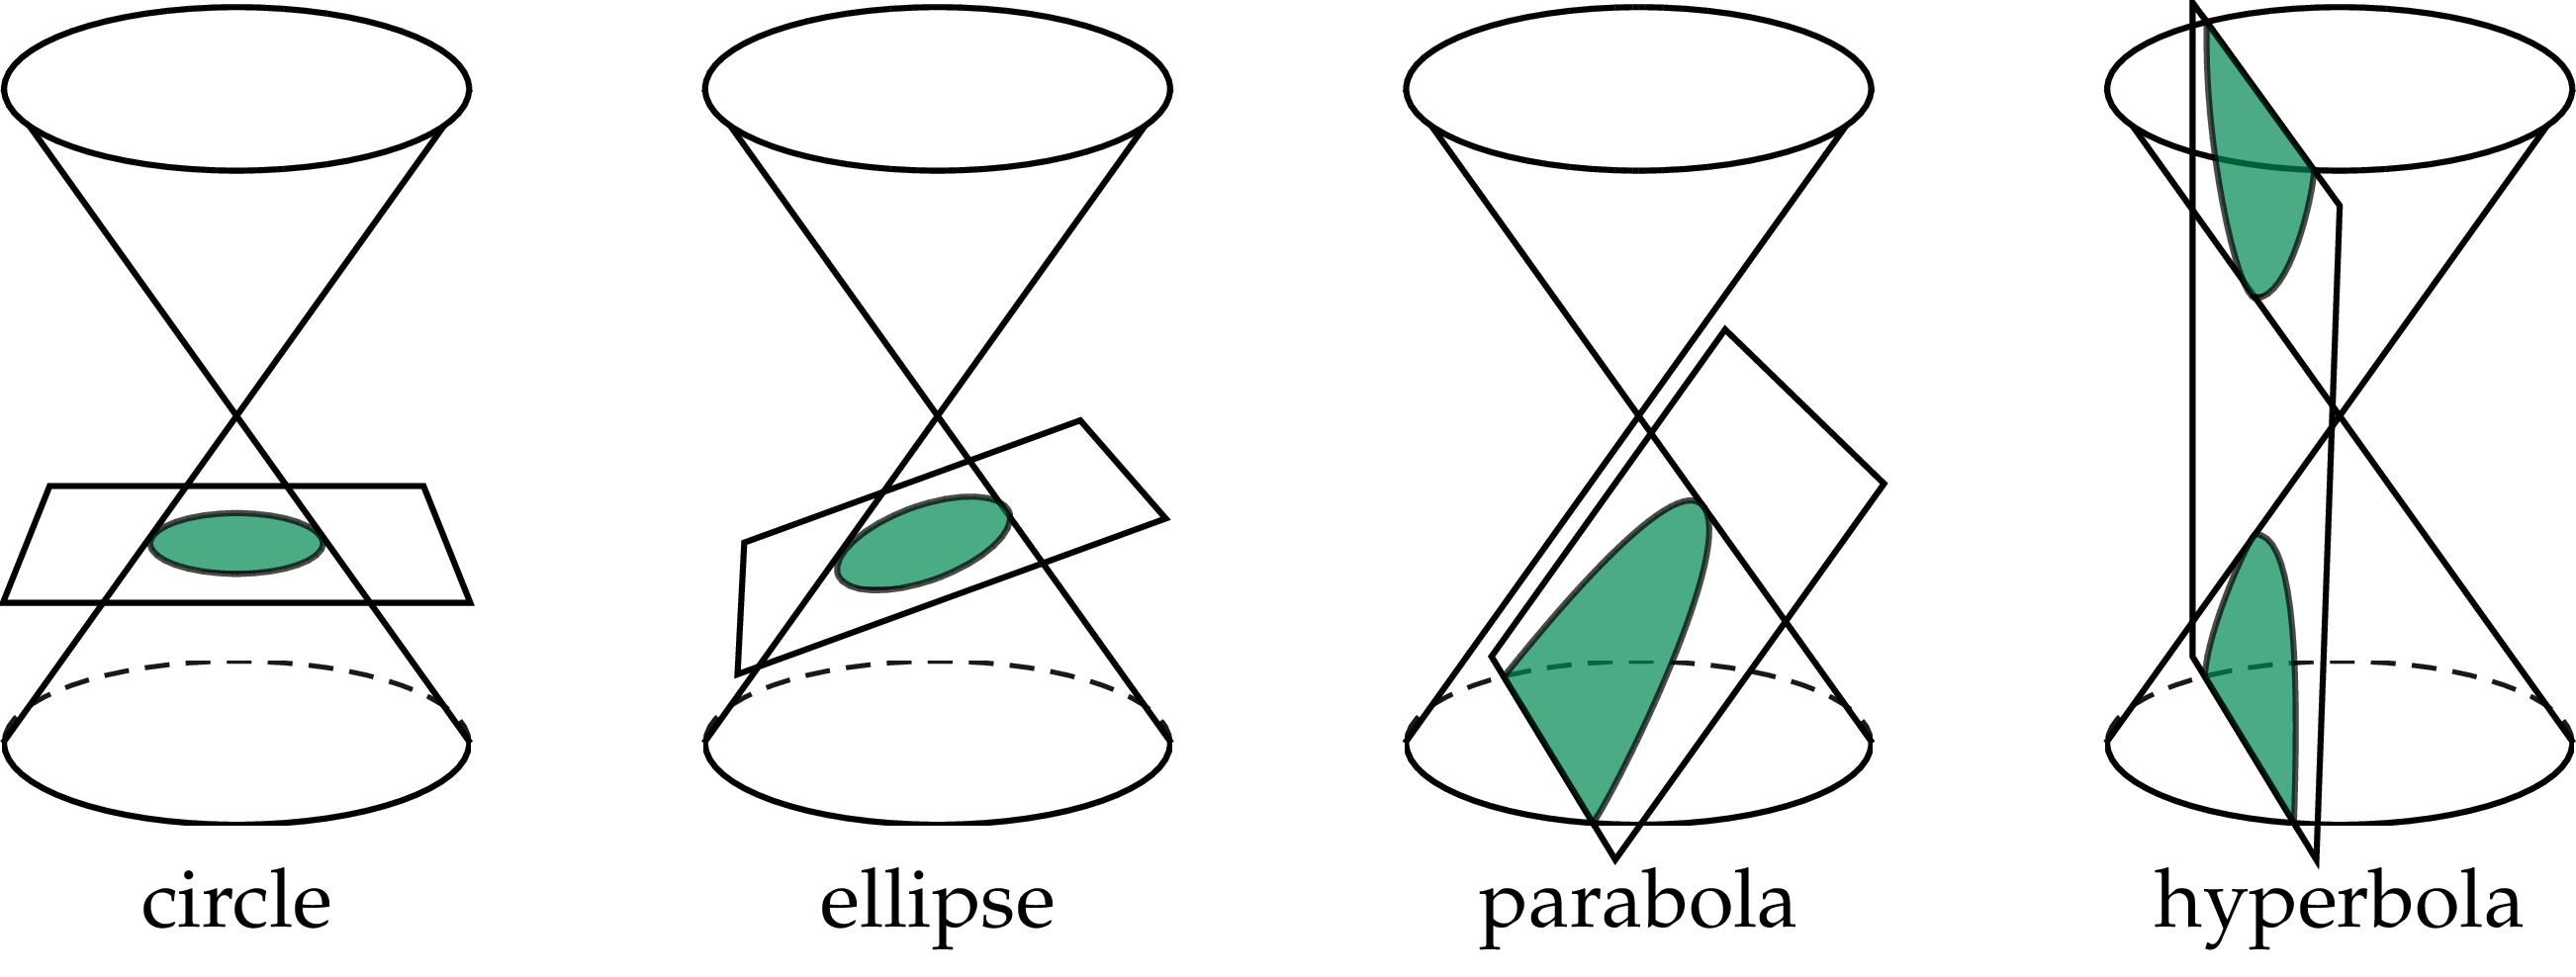
\includegraphics[width=0.8\textwidth]{images/figures/math/conic_sections_four-shapes.png}
			\vspace{-2mm}
			\caption{	Taking slices through a cone at different angles produces different geometric shapes:
					a circle, an ellipse, a parabola, or a hyperbola.\label{fig:conic_sections_four-shapes}}
			
		\end{figure}
	

	\subsection{Conic sections in polar coordinates}

		All four conic sections can be described by the same function in polar coordinates:					
		\[
		  r(\theta) = \frac{q(1+\varepsilon)}{1 + \varepsilon\cos(\theta)}\,,
		\]
		where $q$ is the curve's closest distance to a focal point
		and $\varepsilon$ is the curve's eccentricity.												
		For a circle, $q=R$ (the radius) and the eccentricity parameter is $\varepsilon=0$.
		For an ellipse, $q=a(1-\varepsilon)$ and the eccentricity parameter varies between $0$ and $1$ ($0\leq \varepsilon < 1$).
		Note we include the case $\varepsilon=0$ since a circle is a special case of an ellipse.
		For a parabola, $q=f$ (the focal length) and the eccentricity is $\varepsilon=1$.
		For a hyperbola, $q = a(\varepsilon-1)$ and the eccentricity is $\varepsilon>1$.

		We can use the eccentricity parameter $\varepsilon$ to classify all four curves.
		Depending on the value of $\varepsilon$,
		the equation $r(\theta)$ defines either a circle, an ellipse, a parabola, or a hyperbola.	
		Table~\ref{table:conics} summarizes all our observations regarding conic sections.


		\begin{table}[htb]
		
		\begin{longtable}{lllll} 
		\toprule
		Conic section 	\! 	&  Equation  	\!\!					
		& Polar function	
		&	Eccentricity \!\!\!\!\!\!\!\!\!\!\!\!				\\
		\midrule
		Circle				& $x^2+y^2=R^2$ \; 					& $r(\theta)=R$			& $\varepsilon = 0$								\\
		Ellipse				& $\frac{x^2}{a^2}+\frac{y^2}{b^2}=1$	& $r(\theta)=\frac{a(1-\varepsilon^2)}{1 + \varepsilon\cos(\theta)}$ &	$\varepsilon\!=\!\sqrt{1\!-\!\frac{b^2}{a^2}}\,, \; 0\!\leq\!\varepsilon\!<\!1$\!\!	\\
		Parabola				& $y^2=4fx$						& $r(\theta)=\frac{2f}{1 + \cos(\theta)}$ &	$\varepsilon=1$			 						\\
		Hyperbola			& $\frac{x^2}{a^2}-\frac{y^2}{b^2}=1$	& $r(\theta)=\frac{a(\varepsilon^2-1)}{1 + \varepsilon\cos(\theta)}$ &	$\varepsilon\!=\!\sqrt{1\!+\!\frac{b^2}{a^2}}\,, \; 1\!<\!\varepsilon\!<\!\infty$ \\
		\bottomrule
		\end{longtable}
		\caption{The four conic sections and their eccentricity parameters. \label{table:conics}}
		
		\end{table}


		The motion of the planets is explained by Newton's law of gravitation.
		The gravitational interaction between two bodies always leads one of the two bodies to follow a trajectory described by one of the conic sections
		for which the other body is the focal point.


\section{Math problems}
\label{sec:math_problems}
	
	We've now reached the first section of problems in this book.
	The purpose of these problems is to give you a way to comprehensively practice your math fundamentals.

	
{\small 
	 
\begin{problems}{ch1}

	\vspace*{3mm}


		
	\begin{problem}
		Solve for $x$ in the equation $x^2-9=7$.
		\begin{answer}$x=\pm 4$.\end{answer}
	\end{problem}

	\begin{problem}
		Solve for $x$ in the equation $\cos^{-1}\!\left( \frac{x}{A} \right) - \phi = \omega t$.
		\begin{answer}$x=A\cos(\omega t+\phi)$.\end{answer}
	\end{problem}

	\begin{problem}		\label{mathprob:ch1:fractions2}
		Solve for $x$ in the equation $\frac{1}{x}=\frac{1}{a}+\frac{1}{b}$.	
		\begin{answer}$x=\frac{ab}{a+b}$.\end{answer}
	\end{problem}

	\begin{problem}
		Use a calculator to find the values of the following expressions:
		\fourcol
			\textbf{a)}~$\sqrt[4]{3^3}$
			
			\textbf{b)}~$2^{10}$
			
			\textbf{c)}~$7^{^{\frac{1}{4}}}-10$
			
			\textbf{d)}~$\frac{1}{2}\ln(e^{22})$
		\endfourcol
						\begin{answer}\textbf{a)}~$2.2795$.
					\textbf{b)}~$1024$.
					\textbf{c)}~$-8.373$.
					\textbf{d)}~$11$.\end{answer}
					\end{problem}


	
	\begin{problem} 
		Compute the following expressions involving fractions:
		\threecol
			\textbf{a)}~$\dfrac{1}{2} + \dfrac{1}{4}$
			
			\textbf{b)}~$\dfrac{4}{7} - \dfrac{23}{5}$
			
			\textbf{c)}~$1\frac{3}{4} + 1\frac{31}{32}$
		\endthreecol
		\begin{answer}\textbf{a)}~$\frac{3}{4}$.
					\textbf{b)}~$\frac{-141}{35}$.
					\textbf{c)}~$3\frac{23}{32}$.\end{answer}
		\begin{solution}
			For \textbf{c)}, 
			$1\frac{3}{4} + 1\frac{31}{32} 
				= \frac{7}{4} + \frac{63}{32} 
				= \frac{56}{32} + \frac{63}{32} = \frac{119}{32}=3\frac{23}{32}$.
		\end{solution}
	\end{problem}

	
\end{problems}


} 



